%-----------------------------------------------------------------------------
%
%               Template for sigplanconf LaTeX Class
%
% Name:         sigplanconf-template.tex
%
% Purpose:      A template for sigplanconf.cls, which is a LaTeX 2e class
%               file for SIGPLAN conference proceedings.
%
% Guide:        Refer to "Author's Guide to the ACM SIGPLAN Class,"
%               sigplanconf-guide.pdf
%
% Author:       Paul C. Anagnostopoulos
%               Windfall Software
%               978 371-2316
%               paul@windfall.com
%
% Created:      15 February 2005
%
%-----------------------------------------------------------------------------


%\documentclass[preprint]{sigplanconf}
\documentclass[10pt]{sigplanconf}

% The following \documentclass options may be useful:
%
% 10pt          To set in 10-point type instead of 9-point.
% 11pt          To set in 11-point type instead of 9-point.
% authoryear    To obtain author/year citation style instead of numeric.

\usepackage{yfonts}
\usepackage{amsmath}
\usepackage{amsthm}
\usepackage{amssymb}
%\usepackage{mathpartir}
\usepackage{hyperref}
\usepackage{url}
\usepackage{graphics}
\usepackage{graphicx}
\usepackage{wasysym}
\usepackage{harmony}
\usepackage{marvosym}
\usepackage{multirow}
\usepackage[usenames,dvipsnames]{xcolor}
\usepackage[utopia]{mathdesign}
\usepackage{natbib}
\renewcommand{\UrlBreaks}{\do\/\do\a\do\b\do\c\do\d\do\e\do\f\do\g\do\h\do\i\do\j\do\k\do\l\do\m\do\n\do\o\do\p\do\q\do\r\do\s\do\t\do\u\do\v\do\w\do\x\do\y\do\z}

% ____________________________________________________________
% Listings Package Configuration
% \usepackage[scaled]{beramono}

%\renewcommand*\ttdefault{txtt}
\usepackage[T1]{fontenc}

% This Deep Tex Voodoo is from
%   <http://www.latex-community.org/forum/viewtopic.php?f=5&t=2072>
% It's purpose is to make \lstinline normal size, without affecting
% \lstinputlisting.  It seems to work but I have no idea how or why,
% and I rather hope never to learn.
%\makeatletter
%\lst@AddToHook{TextStyle}{\let\lst@basicstyle\ttfamily\normalsize}
%\makeatother

\begin{document}

\conferenceinfo{SIGBOVIK '17}{Pittsburgh, PA, USA}
\copyrightyear{2017}
\copyrightdata{}

\titlebanner{banner above paper title}        % These are ignored unless
\preprintfooter{short description of paper}   % 'preprint' option specified.

\title{
A Boring Follow-Up Paper to \\
``Which ITG Stepcharts are Turniest?'' \\
Titled, ``Which ITG Stepcharts are Crossoveriest and/or Footswitchiest?'' \\
%That `Boring' Stuff Was Part of the Title, BTW. \\
%So was that. And that, and this too. \\
%You got it all, right? \\
%Or Just, ``More Boring Crap about ITG'', for Short. \\
%Oh, That Was Also Part of the Title.
}
% \subtitle{\em The Randomly-Scoped Lambda Calculus}
% \subtitle{Subtitle Text, if any}

\authorinfo{Ben Blum}{}{bblum@cs.cmu.edu}

\maketitle

\begin{abstract}
	%ITG is a popular dance game in which players step on arrows while listening to music. The arrow patterns, indicated by a {\em stepchart}, may range among any level of complexity and difficulty. Among the many factors contributing to a stepchart's difficulty is how much the player must turn from side to side.
	%Other more obvious factors, such as raw speed, have been well studied in prior work.
	%This paper presents an analytic study of this {\em turniness} factor.
	%We study the turniness of many existing stepcharts, and present a novel (but unsurprising) approach to automatically generating maximally (or minimally) turny charts.
	%Among real-world songs, we find stepcharts with overall turniness ranging from 0\% to 81.33\% of the theoretical maximum.

In which I deliver on last year's promise of future work.

\end{abstract}

\category{D.D.R.}{Exercise and Fitness}{Arcade Dance Games}

\keywords
crossovers, footswitches, jacks, sidefoots


\section{Introduction}

Let's resume right where I left off in my last paper \cite{turniness}, shown in Figure~\ref{fig:you-stutid-fuckass}.
Unlike mainstream conferences, SIGBOVIK doesn't make me waste space repeating all the background material,
and I can just say go read that paper first and get back to me.
It's probably a lot funnier than this one anyway, which is gonna be sort of dry,
and really of interest only to other ITG players who already know what's going on.

\begin{figure}[h]
	\hspace{-2em}\includegraphics[angle=90,width=0.54\textwidth]{../paper.pdf}
	\caption{(okay twist your head to read this)}
	\label{fig:you-stutid-fuckass}
\end{figure}

The TL;DR is that I made a program which figures out how to foot stepcharts in the least crossovery possible way (short of double-stepping everything),
then found which charts ultimately had the most.
The algorithm also naturally identifies footswitches and jacks, %, jacks, forced double-steps, and crossover-footswitches;
and sometimes it's smarter than me in amusing ways.
I put all the goodies in a giant spreadsheet at \url{http://tinyurl.com/crossoveriest},
and the program itself is of course freely available at \url{https://github.com/bblum/sigbovik/blob/master/itg/code/ITG.hs}.



%%%%%%%%%%%%%%%%%%%%%%%%%%%%%%%%%%%%%%%%%%%%%%%%%%%%%%%%%%%%%%%%%%%%%%%%%%%%%%%%

\section{Revisiting Turniness (Flashback Scene)}

Recall Table~\ref{tab:facing} from the last paper, in which I left undefined the facings for $LL$, $DD$, $UU$, and $RR$, the four footswitches.
I show a typical $DD$/$UU$ footswitch pattern in Figure~\ref{fig:fs}(a), and typical $LL$/$RR$ switches (henceforth ``crossover footswitches'') in Figure~\ref{fig:fs}(b).
To step these patterns, the player still alternates feet as usual, but must lift one foot off the repeated arrow before stepping it with her other foot.
Chart authors will often, but not always, include a ``mine cue'' (shown in the figure) to hint that the second foot should switch onto the same arrow.

\begin{table}[t]
	\begin{center}
	\begin{tabular}{cc|cccc}
		& & \multicolumn{4}{c}{Right foot} \\
		& & $\leftarrow$ & $\downarrow$ & $\uparrow$ & $\rightarrow$ \\
		\hline
		\multirow{4}{*}{Left foot}
		%                 L   D   U   R
		& $\leftarrow$  & \bf ? & $UR$ & $UL$ & $U$ \\
		& $\downarrow$  & $DL$ & \bf ? & $L$ & $UL$ \\
		& $\uparrow$    & $DR$ & $R$ & \bf ? & $UR$ \\
		& $\rightarrow$ & $D$ & $DR$ & $DL$ & \bf ? \\

	\end{tabular}
	\end{center}
	\caption{Facing directions.
	%``Crossover'' facings are marked (*), and the ``lateral'' facing is marked ($\dagger$). Note the appealing diagonal symmetry.}
	}
	\label{tab:facing}
\end{table}

\begin{figure}[t]
	\begin{tabular}{c}
	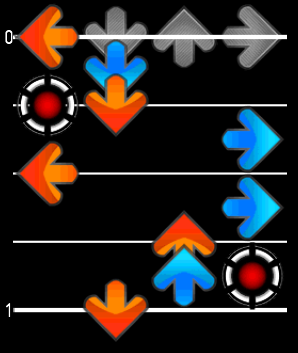
\includegraphics[width=0.13\textwidth]{fs-dd-uu.png} \\
	(a) DD/UU
	\end{tabular}
	\begin{tabular}{c}
	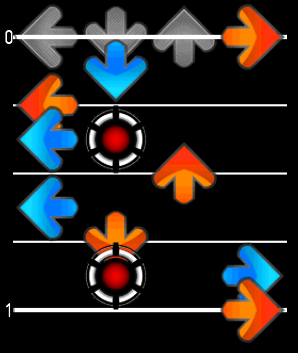
\includegraphics[width=0.13\textwidth]{fs-ll-rr.png} \\
	(b) LL/RR
	\end{tabular}
	\begin{tabular}{c}
	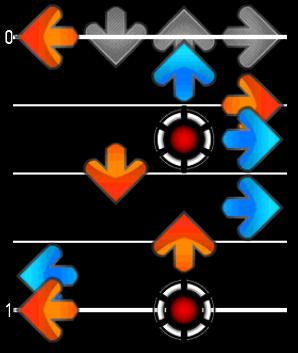
\includegraphics[width=0.13\textwidth]{fs-ll-rr-2.png} \\
	(c) RR/LL
	\end{tabular}
	\caption{Footswitches of various crossoveriness/facing.}
	\label{fig:fs}
\end{figure}

It is tempting to assign the facings $L$, $U$, $U$, and $R$ respectively to the $LL$, $DD$, $UU$, and $RR$ footswitches.
However, Figure~\ref{fig:fs}(c) shows that if a footswitch begins with a crossover on $U$, the facing should be reversed:
the $RR$ footing should face $L$, and $LL$ should face $R$.
``Backwards footswitches'' with $D$ facing are also theoretically possible,
arising from patterns such as $LURDDL$ or $LDRUUL$, although I know of no real-world chart which does this (hmm, tempting...).

Before I realized that, I modified the turniness algorithm \cite{turniness} to face footswitches as above, %the bad way mentioned above,
%to be faced $L$ for $LL$ and so on, as above,
and it surprised me with charts of $\mathcal{T}>2$, in excess of the theoretical maximum!
I show one such chart in Figure~\ref{fig:fs-turniness}(a), in which the step from $LL$ ($\phi=L$) to $UL$ ($\phi=DR$) has individual $\mathcal{T}=3$, and so on for $UL \rightsquigarrow_R UU \rightsquigarrow_L RU \rightsquigarrow_R RR$.
The steps $RR \rightsquigarrow_L LR \rightsquigarrow_R LL$ are both candles ($\mathcal{T}=2$),
resulting overall in $\mathcal{T}=8/3$ for the whole chart.

Indeed, when I further modified the algorithm to force $DD$ switches to face $D$ (i.e., always facing the direction of the repeated arrow),
it produced the chart shown in Figure~\ref{fig:fs-turniness}(b), with overall $\mathcal{T}=3$.
(Note its resemblance to the basic spin pattern, $LDRU$, whose $\mathcal{T}=2$.)

To fairly represent a human player's desire to step in the least turny of ambiguous ways,
I extended the algorithm to provide either the assigned facing, from above, or its polar opposite,
chosen at runtime by whichever is closer to the presequent facing.
This restores the maximum overall chart turniness to $\mathcal{T}=2$,
a new example of which is shown in Figure~\ref{fig:fs-turniness}(c).

However, note that individual steps may still have $\mathcal{T}=3$,
%because after a footswitch's facing is determined, the next step may still ... ?
as shown in Figure~\ref{fig:fs-turniness}(d).
In this example, the step $DL \rightsquigarrow_L LL$ assigns $LL$ to face $L$,
but the subsequent step to $LD$ cannot avoid facing $UR$.
The reason charts still cannot exceed overall $\mathcal{T}=2$ is that
setting up such a situation requires a $\mathcal{T}=1$ step,
which negates the benefit.
A chart could conceivably end right before such a step,
sneaking through some small $\epsilon$ extra turniness \cite{epsilon}
(similar to the case of 270s in \cite{turniness}),
but {\em sustained} average $\mathcal{T}>2$ remains impossible.

Another approach could assign such a footswitch the opposite footing of the previous facing,
%regardless of the switch arrow itself;
so in this case the $LL$ would face $UL$, and each step would have exactly $\mathcal{T}=2$.
Anyway, remember that all-candle switch stream from (c). We'll see it again soon.

\begin{figure}[t]
	\begin{center}
	\begin{tabular}{c}
	\begin{tabular}{c}
	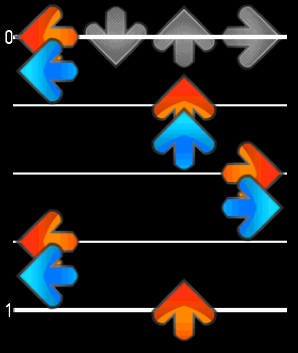
\includegraphics[width=0.13\textwidth]{fs-turniness-8-3.png} \\
	(a) $\mathcal{T}=8/3$(?)%\stackrel{?}{=}8/3$
	\end{tabular}
	\begin{tabular}{c}
	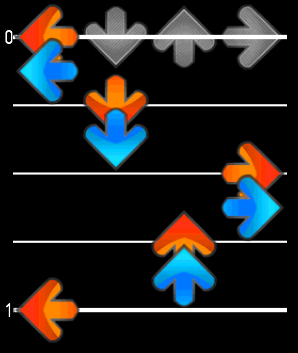
\includegraphics[width=0.13\textwidth]{fs-turniness-3.png} \\
	(b) $\mathcal{T}=3$(?)%\stackrel{?}{=}3$
	\end{tabular}
	\\
	\\
	\begin{tabular}{c}
	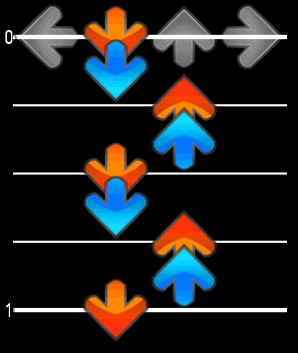
\includegraphics[width=0.13\textwidth]{fs-turniness-2.png} \\
	(c) $\mathcal{T}=2$.
	\end{tabular}
	\begin{tabular}{c}
	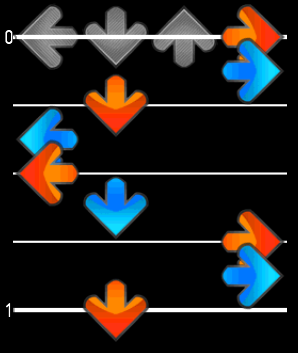
\includegraphics[width=0.13\textwidth]{fs-turniness-2-plus-epsilon.png} \\
	(d) $\mathcal{T}=2+\epsilon$.
	\end{tabular}
	\end{tabular}
	\end{center}
	\caption{The turniest footswitch patterns. (a) and (b) are false positives (see prose), while (c) and (d) provide theoretically maximal turniness.}
	\label{fig:fs-turniness}
\end{figure}


% dont forget
% http://dancedancerevolutionddr.wikia.com/wiki/Afronova_walk

%%%%%%%%%%%%%%%%%%%%%%%%%%%%%%%%%%%%%%%%%%%%%%%%%%%%%%%%%%%%%%%%%%%%%%%%%%%%%%%%

\newcommand\hilight[2]{\color{#1}#2\color{black}}
\definecolor{pink}{RGB}{128,0,192}
\definecolor{orange}{RGB}{192,96,0}
\definecolor{olivegreen}{RGB}{0,127,32}
\definecolor{brickred}{RGB}{192,0,0}
\definecolor{commentblue}{RGB}{0,128,192}

\begin{figure*}[t]
\begin{center}
\begin{tabular}{l}
	\texttt{\hilight{orange}{data}~\hilight{olivegreen}{Step}~= \hilight{brickred}{L}~| \hilight{brickred}{D}~| \hilight{brickred}{U}~| \hilight{brickred}{R}~| \hilight{brickred}{Jump}~\hilight{orange}{deriving}~\hilight{olivegreen}{Eq}} \\
\texttt{} \\
\texttt{\hilight{orange}{data}~\hilight{olivegreen}{AnalysisState}~= \hilight{brickred}{S}~\{ steps :: \hilight{olivegreen}{Int}, xovers :: \hilight{olivegreen}{Int}, switches :: \hilight{olivegreen}{Int}, jacks :: \hilight{olivegreen}{Int},} \\
\texttt{~~~~~~~~~~~~~~~~~~~~~~~~ lastStep :: \hilight{olivegreen}{Maybe}~\hilight{olivegreen}{Step}, doubleStep :: \hilight{olivegreen}{Bool}, lastFlip :: \hilight{olivegreen}{Bool},} \\
\texttt{~~~~~~~~~~~~~~~~~~~~~~~~ lastFoot :: \hilight{olivegreen}{Bool}, stepsLR :: [\hilight{olivegreen}{Bool}] \}} \\
\texttt{} \\
\texttt{\hilight{pink}{commitStream}~:: \hilight{olivegreen}{AnalysisState}~-> \hilight{olivegreen}{AnalysisState}} \\
\texttt{\hilight{pink}{commitStream}~s = s \{ xovers~~ = xovers~~ s + \hilight{orange}{if}~f \hilight{orange}{then}~ns - nx \hilight{orange}{else}~nx, } \\
\texttt{~~~~~~~~~~~~~~~~~~~~ switches = switches s + \hilight{orange}{fromEnum}~(f == lastFlip s \&\& doubleStep s), } \\
\texttt{~~~~~~~~~~~~~~~~~~~~ jacks~~~~= jacks~~~~s + \hilight{orange}{fromEnum}~(f /= lastFlip s \&\& doubleStep s), } \\
	\texttt{~~~~~~~~~~~~~~~~~~~~ lastFlip = f, stepsLR = \hilight{brickred}{[]}~\}} \\
\texttt{~~~~\hilight{orange}{where}~ns = \hilight{orange}{length}~\$~stepsLR s} \\
\texttt{~~~~~~~~~~nx = \hilight{orange}{length}~\$ \hilight{orange}{filter not}~\$ stepsLR s} \\
\texttt{~~~~~~~~~~\hilight{commentblue}{-{}- if more than half the L/R steps in this stream were crossed over,}} \\
\texttt{~~~~~~~~~~\hilight{commentblue}{-{}- then we got the footing backwards and need to flip the stream.}} \\
\texttt{~~~~~~~~~~\hilight{commentblue}{-{}- as a tiebreaker, flip if the chart is already more jacky than}} \\
\texttt{~~~~~~~~~~\hilight{commentblue}{-{}- footswitchy, i.e., if past streams flipped more often than not.}} \\
\texttt{~~~~~~~~~~f = nx * 2 > ns || nx * 2 == ns \&\& ((switches s > jacks s) == lastFlip s)} \\
\texttt{} \\
\texttt{\hilight{pink}{analyzeStep}~:: \hilight{olivegreen}{AnalysisState}~-> \hilight{olivegreen}{Step}~-> \hilight{olivegreen}{AnalysisState}} \\
\texttt{\hilight{pink}{analyzeStep}~s step} \\
\texttt{~~~~\hilight{commentblue}{-{}- a jump resets the footing, so the next step can be stepped with either}} \\
\texttt{~~~~\hilight{commentblue}{-{}- foot. commit the stream so far to treat it separately from what follows.}} \\
\texttt{~~~~\hilight{commentblue}{-{}- bracket-jumps are, of course, future work.}} \\
\texttt{~~~~| step == \hilight{brickred}{Jump}~= (\hilight{pink}{commitStream}~s) \{ lastStep = \hilight{brickred}{Nothing}, doubleStep = \hilight{brickred}{False}~\}} \\
\texttt{~~~~\hilight{commentblue}{-{}- two steps on the same arrow might be a jack, or might be a footswitch.}} \\
\texttt{~~~~\hilight{commentblue}{-{}- to figure out which, commit the stream so far, and begin a new stream}} \\
\texttt{~~~~\hilight{commentblue}{-{}- whose footing will retroactively determine how to foot this step.}} \\
\texttt{~~~~\hilight{commentblue}{-{}- also, unlike jumps, this step gets counted as part of the next stream.}} \\
\texttt{~~~~| lastStep s == \hilight{brickred}{Just}~step = stream (\hilight{pink}{commitStream}~s) \{ doubleStep = \hilight{brickred}{True}~\}} \\
\texttt{~~~~\hilight{commentblue}{-{}- a normal streamy step.}} \\
	\texttt{~~~~| \hilight{orange}{otherwise}~= stream s} \\
\texttt{~~~~\hilight{orange}{where}~foot = \hilight{orange}{not}~\$ lastFoot s} \\
\texttt{~~~~~~~~~~\hilight{commentblue}{-{}- record whether we stepped on a matching or crossed-over L/R arrow.}} \\
\texttt{~~~~~~~~~~addStep ft \hilight{brickred}{L}~steps = steps ++ [ft]} \\
\texttt{~~~~~~~~~~addStep ft \hilight{brickred}{R}~steps = steps ++ [\hilight{orange}{not}~ft]} \\
\texttt{~~~~~~~~~~addStep ft \_ steps = steps \hilight{commentblue}{-{}- U/D don't help to determine L/R footing.}} \\
\texttt{~~~~~~~~~~stream s = s \{ steps = steps s + \hilight{brickred}{1}, lastStep = \hilight{brickred}{Just}~step, lastFoot = foot,} \\
\texttt{~~~~~~~~~~~~~~~~~~~~~~~~ stepsLR = addStep foot step \$ stepsLR s \} } \\
\texttt{} \\
\texttt{\hilight{pink}{analyze}~:: [\hilight{olivegreen}{Step}] -> \hilight{olivegreen}{AnalysisState}} \\
	\texttt{\hilight{pink}{analyze}~= \hilight{pink}{commitStream}~. \hilight{orange}{foldl}~\hilight{pink}{analyzeStep}~(\hilight{brickred}{S 0 0 0 0}~\hilight{brickred}{Nothing}~\hilight{brickred}{False}~\hilight{brickred}{False}~\hilight{brickred}{False}~\hilight{brickred}{[]}) } \\
\end{tabular}
\end{center}
\caption{it's pseudocode lol}
\label{fig:pseudocode-lol}
\end{figure*}


\section{Existing Chart Analysis}

%%%%%%%%%%%%%%%%%%%%%%%%%%%%%%%%%%%%%%%%%%%%%%%%%%%%%%%%%%%%%%%%%%%%%%%%%%%%%%%%

%\section{A Bit More on Turniness}

%%%%%%%%%%%%%%%%%%%%%%%%%%%%%%%%%%%%%%%%%%%%%%%%%%%%%%%%%%%%%%%%%%%%%%%%%%%%%%%%

\section{Experimental Results}

% TODO: Put a * on charts where you're going to put a pict of mario man
% TODO: Put a dagger on footswitch charts where the footing is a clever reinterpretation, rather than intended

% TODO: Make a special mention of sandstorm and put a pict of mario man
% TODO: put the above in an honourable mention subsection, and also mention the slow train and sidefoots

\begin{figure}[t]
	\begin{center}
		\small
	\begin{tabular}{r|l|l|c|c}
		\bf Ft. & \bf Name & \bf Pack & \bf \#XO & \bf XO\% \\
		\hline
		\multicolumn{5}{c}{\em no 8s- with $\ge$100 XOs} \\
		 9 & MAX Forever              & CuoReNeRo MeGaPacK    & \bf 107 & \em 8.7 \\
		10 & J-PARA SUPER MEGAMIX     & CuoReNeRo MeGaPacK    & \bf 141 & \em 3.9 \\
		11 & Somebody That I Used To Know & Best of Gazebo    & \bf 114 & \em 11.9 \\
		12 & Credens Justitiam        & Stuff B Likes         & \bf 136 & \em 12.4 \\
		13 & Banshee Strikes          & VocaJawnz             & \bf 152 & \em 10.2 \\
		14 & Slow Down                & Sexuality Violation 2 & \bf 160 & \bf 13.3 \\
		15 & MAX Forever              & CuoReNeRo MeGaPacK    & \bf 101 & \em 4.2 \\
		\multicolumn{5}{c}{\em no 16s-20s with $\ge$100 XOs} \\
		21 & Teenage Dream            & Sexuality Violation 2 & \bf 280 & \bf 11.8 \\
	\end{tabular}
	\end{center}
	\caption{Charts with the most total crossovers (XOs).}
\end{figure}
\begin{figure}[t]
	\begin{center}
		\small
	\begin{tabular}{r|l|l|c|c}
		\bf Ft. & \bf Name & \bf Pack & \bf \#XO & \bf XO\% \\
		\hline
		 4 & DAM DIRIRAM              & DDR 3rdMIX            & \em  30 & \bf 27.3 \\
		 5 & STRICTLY BUSINESS        & DDR 1st               & \em  33 & \bf 21.4 \\
		 6 & STRICTLY BUSINESS        & DDR 1st               & \em  38 & \bf 20.9 \\
		 7 & MOBO$\star$MOGA          & DDR EXTREME           & \em  37 & \bf 17.3 \\
		 8 & PARANOiA                 & DDR 1st               & \em  58 & \bf 19.6 \\
		 9 & Dazzlin Darlin           & r21twins              & \em  76 & \bf 22.0 \\
		10 & Enchanted Journey        & ITG Rebirth           & \em  78 & \bf 19.3 \\
		11 & Lune Noir                & r21freak Friendship   & \em  58 & \bf 13.4 \\
		12 & Winnipeg is Fucking Over & best of r21freak ii   & \em 122 & \bf 14.3 \\
		13 & The Sampling Paradise    & The Paradise Sampler  & \em 139 & \bf 15.6 \\
		14 & Slow Down                & Sexuality Violation 2 & \bf 160 & \bf 13.3 \\
		\multicolumn{5}{c}{\em no 15s-20s with $\ge$10\% XO} \\
		21 & Teenage Dream            & Sexuality Violation 2 & \bf 280 & \bf 11.8 \\
	\end{tabular}
	\end{center}
	\caption{Charts with the highest percentage of crossovers among total steps.}
\end{figure}
\begin{figure}[t]
	\begin{center}
		\small
	\begin{tabular}{r|l|l|c|c}
		\bf Ft. & \bf Name & \bf Pack & \bf \#FS & \bf FS\% \\
		\hline
		\multicolumn{5}{c}{\em no 5s- with $\ge$50 FSs} \\
		 6 & Sweat Shop       & ITG Rebirth 2 Beta    & \bf  56 & \bf 18.2 \\
		\multicolumn{5}{c}{\em no 7s-9s with $\ge$50 FSs} \\
		10 & Eat 'Em Up!      & Mute Sims 5           & \bf  54 & \em  9.0 \\
		11 & Nemeton          & The Legend of Zim 4   & \bf  97 & \em 10.3 \\
		12 & Nemeton          & Subluminal            & \bf 140 & \bf 14.8 \\
		13 & Love Is Eternity & Subluminal            & \bf 140 & \bf 16.8 \\
		14 & Switch           & Getty                 & \bf 347 & \bf 15.7 \\
		15 & Danse Macabre    & Aoreo's Ariginals     & \bf 201 & \em 12.2 \\
		16 & Weird Science    & Stamina Showcase      & \bf  61 & \em  1.8 \\
		\multicolumn{5}{c}{\em no 17s+ with $\ge$50 FSs} \\
	\end{tabular}
	\end{center}
	\caption{Charts with the most total footswitches (FSs).}
\end{figure}
\begin{figure}[t]
	\begin{center}
		\small
	\begin{tabular}{r|l|l|c|c}
		\bf Ft. & \bf Name & \bf Pack & \bf \#FS & \bf FS\% \\
		\hline
		%\multicolumn{5}{c}{\em no <6s with >50 FSs} \\
		 3 & Sweat Shop       & ITG Rebirth 2 Beta    & \em  26 & \bf 15.3 \\
		 4 & MAKE IT BETTER   & DDR 2ndMIX            & \em  26 & \bf 20.0 \\
		\multicolumn{5}{c}{\em no 5s with $\ge$10\% FS} \\
		 6 & Sweat Shop       & ITG Rebirth 2 Beta    & \bf  56 & \bf 18.2 \\
		 7 & 5.1.1            & DDR MAX               & \em  13 & \bf 12.9 \\
		\multicolumn{5}{c}{\em no 8s with $\ge$10\% FS} \\
		 9 & PARANOiA KCET    & DDR 2ndMIX            & \em  33 & \bf 10.2 \\
		10 & Delhi Ill        & Mute Sims 6           & \em  40 & \bf 11.6 \\
		11 & Sweat Shop       & ITG Rebirth 2 Beta    & \em  75 & \bf 11.8 \\
		12 & Nemeton          & Subluminal            & \bf 140 & \bf 14.8 \\
		13 & Love Is Eternity & Subluminal            & \bf 140 & \bf 16.8 \\
		14 & Switch           & Getty                 & \bf 347 & \bf 15.7 \\
		15 & Flames of the Sky & fort rapids vii      & \em 172 & \bf 16.5 \\
		\multicolumn{5}{c}{\em no 16s+ with $\ge$10\% FS} \\
	\end{tabular}
	\end{center}
	\caption{Charts with the highest percentage of footswitches among total steps.}
\end{figure}
\begin{figure}[t]
	\begin{center}
		\small
	\begin{tabular}{r|l|l|c|c}
		\bf Ft. & \bf Name & \bf Pack & \bf \#XF & \bf XF\% \\
		\hline
		\multicolumn{5}{c}{\em no 8s- with $\ge$12 XFs} \\
		 9 & Dr. Boom-Bombay   & fort rapids vii            & \bf 18 & 4.0 \\
		10 & Toxic             & Sexuality Violation 2      & \bf 12 & 1.5 \\
		11 & Heart Shooter     & VocaJawnz                  & \bf 44 & 5.1 \\
		12 & Beautiful Synergy & Keyboard Collaboration III & \bf 14 & 3.2 \\
		13 & Toxic             & Sexuality Violation 2      & \bf 12 & 1.2 \\
		14 & Fancy Footwork    & Cirque du Zeppelin         & \bf 40 & 4.2 \\
		\multicolumn{5}{c}{\em no 14s+ with $\ge$12 XFs} \\
	\end{tabular}
	\end{center}
	\caption{Charts with the most crossover footswitches (XFs). (Here I chose 12 as the cut-off because below that are a bunch of false-positives from DDR.)}
\end{figure}

\section{Conclusion}

Please accept our paper.
We worked hard on it.

%%%%%%%%%%%%%%%%%%%%%%%%%%%%%%%%%%%%%%%%%%%%%%%%%%%%%%%%%%%%%%%%%%%%%%%%%%%%%%%%

\bibliographystyle{abbrvnat}
\bibliography{citations}

\end{document}
